\documentclass[10pt, hyperref={pdfpagelabels=false}]{beamer}

\usepackage{tikz, verbatim, enumitem}

\usetikzlibrary{decorations}
\usetikzlibrary{backgrounds}
\usetikzlibrary{patterns}
\usetikzlibrary{snakes}
\usetikzlibrary{shapes}
\usetikzlibrary{positioning, shapes.geometric, arrows.meta}
\usetikzlibrary{arrows,automata}

\setlength{\parindent}{0pt}
\setlength{\parskip}{1.3ex}

\title{Securing the Transport Layer}
\author{Michael Brockway}
\date{\today}

\setlist[enumerate]{itemsep=0mm}
\setitemize{label=\usebeamerfont*{itemize item}
  \usebeamercolor[fg]{itemize item}
  \usebeamertemplate{itemize item}}

\begin{document}

\begin{frame}
\titlepage
\end{frame}

\begin{frame}
\frametitle{Introduction}
\begin{center}
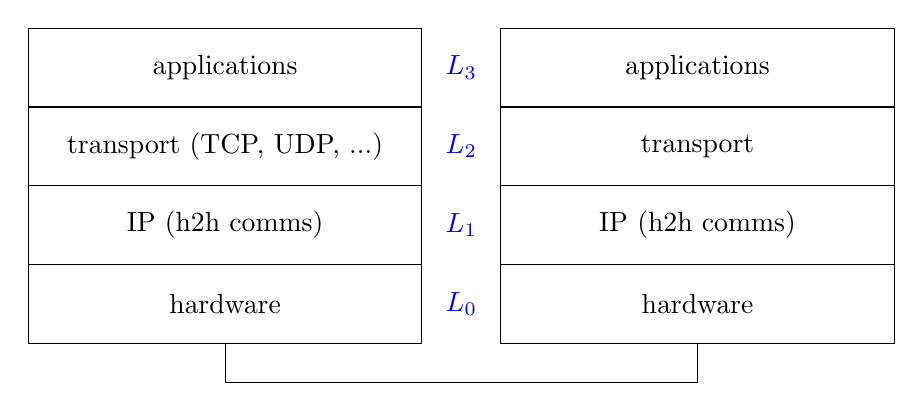
\begin{tikzpicture} [minimum height=1, draw]
  \draw (0,6) rectangle (5,7); \draw (2.5,6.5) node {applications}; 
  \draw (0,5) rectangle (5,6); \draw (2.5,5.5) node {transport (TCP, UDP, ...)}; 
  \draw (0,4) rectangle (5,5); \draw (2.5,4.5) node {IP (h2h comms)}; 
  \draw (0,3) rectangle (5,4); \draw (2.5,3.5) node {hardware}; 

  \draw (6,6) rectangle (11,7); \draw (8.5,6.5) node {applications}; 
  \draw (6,5) rectangle (11,6); \draw (8.5,5.5) node {transport};
  \draw (6,4) rectangle (11,5); \draw (8.5,4.5) node {IP (h2h comms)}; 
  \draw (6,3) rectangle (11,4); \draw (8.5,3.5) node {hardware}; 

  \draw (5.5,3.5) node[color=blue] {$L_0$}; \draw (5.5,4.5) node[color=blue] {$L_1$};   
  \draw (5.5,5.5) node[color=blue] {$L_2$}; \draw (5.5,6.5) node[color=blue] {$L_3$};   

  \draw (2.5,3) -- (2.5,2.5) -- (8.5,2.5) -- (8.5,3);
\end{tikzpicture}
\end{center}

Applications that have to communicate data use transport layer services which use IP services, which use network hardware connected by data communications hardware.

The line connecting the two stacks is a \emph{communications channel} using wire, wireless (two-way radio), fiber-optics or some combination.
\end{frame}

\begin{frame}
\frametitle{Introduction - the problem}
\begin{itemize}
\item In the basic setup, a third party could connect to the physical data communications channel and `eavesdrop'.
\item Alternatively, the third party can interpose themselves between the original parties (tampering with the physical coonections or wireless channels), intercept data packets and tamper with them...
\item or destroy them... 
\item or inject data packets purporting to come from one of the original parties. 
\item Third parties can flood the channel with junk messages making it impossible for the original partis to function - (distributed) \emph{denial of service} attack.
\end{itemize} 

The applications need some defence against these.

DoS attacks are protected against by \emph{firewalls} -- processes that control ingress or egress of data packets from one network to another: these are often built-in to routers.

The other problems can be dealt with in a more general fashion ...
\end{frame}

\begin{frame}
\frametitle{Transport layer security requirements}
Fundamentally, applications communicate with one another,
\begin{itemize}
\item an application needs to know that a data packet cannot be read by unauthorised third parties - \emph{\color{blue}privacy} or \emph{\color{blue}confidentiality}.
\item It needs to know it genuinely came from the network address given in the packet and was not injected by an imposter - \emph{\color{blue}authenticity}.
\item It needs to know the data contents are as sent and have not been tampered with - \emph{\color{blue}integrity}.
\end{itemize} 

The \emph{assurances} are met by software sitting between the transport and application layers.
\end{frame}

\begin{frame}
\frametitle{Transport layer security - basic setup}
\begin{center}
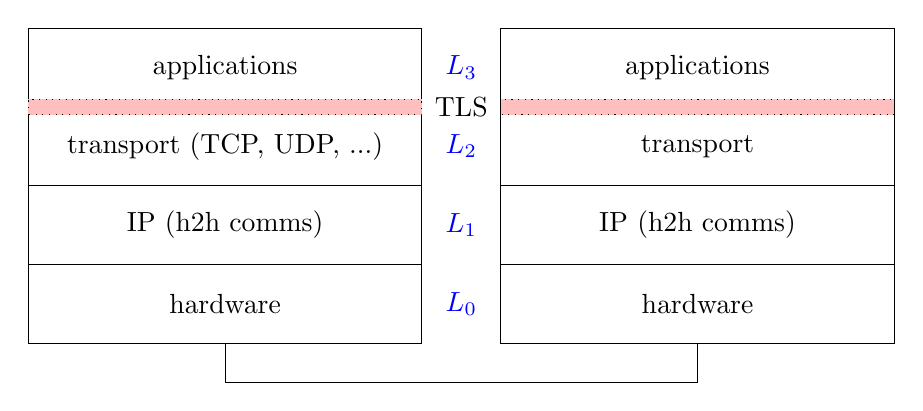
\begin{tikzpicture} [minimum height=1, draw]
  \draw (0,6) rectangle (5,7); \draw (2.5,6.5) node {applications}; 
  \draw (0,5) rectangle (5,6); \draw (2.5,5.5) node {transport (TCP, UDP, ...)}; 
  \draw (0,4) rectangle (5,5); \draw (2.5,4.5) node {IP (h2h comms)}; 
  \draw (0,3) rectangle (5,4); \draw (2.5,3.5) node {hardware}; 

  \draw (6,6) rectangle (11,7); \draw (8.5,6.5) node {applications}; 
  \draw (6,5) rectangle (11,6); \draw (8.5,5.5) node {transport};
  \draw (6,4) rectangle (11,5); \draw (8.5,4.5) node {IP (h2h comms)}; 
  \draw (6,3) rectangle (11,4); \draw (8.5,3.5) node {hardware}; 

  \draw (5.5,3.5) node[color=blue] {$L_0$}; \draw (5.5,4.5) node[color=blue] {$L_1$};   
  \draw (5.5,5.5) node[color=blue] {$L_2$}; \draw (5.5,6.5) node[color=blue] {$L_3$};   

  \draw (2.5,3) -- (2.5,2.5) -- (8.5,2.5) -- (8.5,3);

  \draw[dotted, fill=pink] (0,5.9) rectangle  (5,6.1);
  \draw[dotted, fill=pink] (6,5.9) rectangle (11,6.1);
  \draw (5.5,6) node {TLS};
\end{tikzpicture}
\end{center}

\emph{Transport-layer Security} (TLS) is a `thin' software layer sitting between the transport and application layers in the original TCP/IP stack.
\end{frame}

\begin{frame}
\frametitle{Transport layer security - basic setup}
TLS is designed to provide the required assurances:
\begin{itemize}
\item A data packet cannot be read by unauthorised third parties: \emph{\color{blue}confidentiality} is assured use of a suitable \emph{encryption} scheme. Data is encrypted before it is sent and decrypted when it received; only the legitimately communicating parties are able do this.
\item A data packet comes with a \emph{digital signature} which can be \emph{authenticated} at the receiving end. Suitable digital signature schemes make it hard for a third party to fake a digital signature and thus assure \emph{\color{blue}authenticity}.
\item The \emph{\color{blue}integrity} of a message is assured by using a \emph{cryptographic hash function}. This function generates a \emph{message digest} or \emph{message authentication code} (MAC) which can be generated at the sending end and attached to the message; it is generated at the receiving end also, and the two values compared. Good hash functions make it difficult for a third party to alter the message while keeping the hash value the same.
\end{itemize} 
\end{frame}

\begin{frame}
\frametitle{Message and hash functions}
A \emph{hash function} takes as input a (possibly very long) sequence of bytes and returns a \emph{hash value}, a number in a fixed range.
\begin{itemize}
\item For instance SHA256 returns a 256-bit number: in effect a number in the range 0 ... $2^{256}-1$.
\end{itemize} 

This is similar to the hash functions which support hash-tables of objects. What is special about a cryptographic hash function is that
\begin{itemize}
\item A small change in the input message (the byte sequence) always produces a big jump in the hash value;
\item It is computationally infeasible to reverse-engineer hash values: to contrive a message whose hash is a given value;
\item It is computationally infeasible to contrive two messages which give equal hash values.
\end{itemize} 

A \emph{\color{blue}collision-resistant} hash function is one with the first two of these properties. If it has all three properties it is \emph{\color{blue}strongly collision-resistant}.
\end{frame}

\begin{frame}
\frametitle{Message and hash functions}

Thus, an attempt to tamper with message data will alter the hash. If a particular hash value is expected by the receiver, tampering will be detected.
\begin{itemize}
\item Contriving two messages that hash to the same value is a \emph{birthday attack}: so called because the probability that in a group of $n$ people, two will have a birthday on the same day is over 0.5 when $n > 23$. (See the wikipedia article on birthday attacks!) 
\item A strongly collision resistent hash function can thus be used to foil birthday attacks.
\end{itemize} 

Usual TLS practice is
\begin{itemize}
\item The sender computes the hash of the message and appends the hash value to the message;
\item the message+hash is encrypted and sent;
\item the receiver decrypts the data and splits off the hash value;
\item the receiver computes the hash of the received message and compares it with the received hash value.
\item Tampering will inevitably have cause a mismatch.
\end{itemize} 
\end{frame}

\begin{frame}
\frametitle{Encryption}
Encryption algorithms are in the public domain; their security lies in being \emph{key-driven}
\begin{itemize}
\item The typical scheme is {\color{blue}$c = E(k,m)$; $m = D(k',c)$;} 
\item $m$ is the \emph{\color{blue}plain-text} message (byte sequence), $c$ is the \emph{\color{blue}cipher-text}.
\item $E$ is the \emph{\color{blue}encryption} function which takes a \emph{\color{blue}key} as well as the message. 
\item $D$ is the companion \emph{\color{blue}decryption} function which takes a \emph{\color{blue}key} as well as the ciphertext.
\item $E, D$ are \emph{\color{blue}inverses}: provided $k'$ is the decryption key corresponding to encryption key $k$, then
\item {\color{brown}$\forall m: D(k', E(k,m)) = m$} and {\color{brown}$\forall c: E(k, D(k',c)) = c$}
\item $E, D$ are publicly known; but no-one can infer $m$ from $c$ without knowing $k'$.
\end{itemize} 
Thus in TLS, 
\begin{itemize}
\item the sender will send $E(k,m+h(m)) = c$ [$m$ = message, $h(m)$ = hash] 
\item the receiver will receive $c$ and decrypt: $D(k',c) = m'+h'$
\item the receiver will check that $h(m') = h'$ to verify integrity. 
\end{itemize} 
\end{frame}

\begin{frame}
\frametitle{Encryption}
A \emph{\color{blue}symmetric} encryption system is one with $k' = k$: the same key is used in encryption and decryption: it is shared between sender and receiver. Seems like a simplification but ...
\begin{itemize}
\item If a server, say, at PayPal, has to share pairs of keys with millions of customers, this is a massive management problem;
\item How can it \emph{agree} a shared key with each customer without an eaveropper discovering it?
\item There has to be a different key with each customer (why?)
\end{itemize}

An \emph{\color{blue}asymmetric} encryption system has $k' \ne k$:
\begin{itemize}
\item Now PayPal can publish its encryption key $k_{PP}$. PayPal's decription key $k'_{PP}$ cannot be inferred; so anyone can send a message privately to PayPal and only PayPal can read it.
\item PayPal's $k_{PP}$ is its \emph{\color{blue}public key}; $k_{PP}'$ is its \emph{\color{blue}private key}. Assymetric cryptosystems are more usually called \emph{\color{blue}public key cryptosystems}.   
\end{itemize}
\end{frame}

\begin{frame}
\frametitle{Encryption}
\begin{itemize}
\item PayPal customer Fred also has a public key $k_F$ and a private key $k'_F$.
\item A message $PP \rightarrow F$ is encrypted by PP with $k_F$ (OK because $k_F$ is public!) and recovered by F with $k'_F$; 
\item A message $F \rightarrow PP$ is encrypted by F with $k_{PP}$ and recovered by PP with $k'_{PP}$.
\end{itemize}

We seem to have covered message integrity and confidentiality. What about authentication? Our public-key cryptographic system can be used for this too.
\begin{itemize}
\item PayPal can append its messages with its \emph{\color{blue}digital signature} $sig = D(k'_{PP},``PayPal")$.
\item The hash(msg+sig) is computed and appended;
\item The whole is encrypted: $E(k_F, (msg+sig+hash) = c$ and sent to Fred
\item Fred decrypts: $D(k'_F,c)$ and recovers msg+sig+hash
\item Fred extracts the hash and compares it to locally computed $hash(msg+sig)$ to check integrity.
\end{itemize}
\end{frame}

\begin{frame}
\frametitle{Encryption}
\begin{itemize}
\item To Fred, the message looks like plain text but the signature looks funny because if it is authentic, it is $D(k'_{PP},``PayPal")$.
\item Fred can check this by applying PP's public key: $E(k_{PP},D(k'_{PP},``PayPal"))$ - should get ``PayPal" in plain text.
\item This works because not only {\color{brown}$\forall m: D(k', E(k,m)) = m$} (encryption followed by decryption) but also {\color{brown}$\forall c: E(k, D(k',c)) = c$}.
\end{itemize}

The public-key system is used with the roles of $E(k,-)$ and $D(k',-)$ reversed to do authentication.

Of course, all this work is done by PayPal's server and Fred's web browser and/or email client: not by an actual Fred. 
\end{frame}

\begin{frame}
\frametitle{Digital Certificates}
How does Fred know the message from PayPal is really from PayPal and not from a `man in the middle' masquerading as PayPal?
\begin{itemize}
\item PayPal's public key $k_{PP}$ is registered with a trusted \emph{\color{blue}certificate authority}.
\item Fred's browser will verify $k_{PP}$ with this authority before using it to check the authenticity of the message.
\end{itemize}
\end{frame}

\begin{frame}
\frametitle{Re-enter symmetric cryptosystems}
There is a problem with the scheme outlined so far. All current public key systems are very strong, but also slow: to slow for bulk encryption of megabytes of data in reasonable time.

Symmetric systems such as AES are 1000 or more times as fast. Unfortuately, the shared keys are impossible to manage on a large scale.

TLS therefore uses a hybrid system: a session between (say) PayPal and Fred
\begin{itemize}
\item start with an initial `handshake' using a public key cryptosystem as above.
\item Then a shared key is agreed for use in an agreed symmetric cryptosystem for the duration of the session.
\item This negotion is kept private by use of the public-key system. There are also other `key agreement protocols' such as Diffie-Hellman key agreement.
\item From time to time during a long session, a new session key will be negotiated.
\end{itemize}
\end{frame}

\begin{frame}
\frametitle{TLS practicalities}
Examples of hash functions and cryptosystems actually used in transport-layer security will be outlined in the next two lectures. The last few slides here give a brief outline of the structure of TLS.

TLS originally developed from from SLL.
\small
\begin{itemize} 
\item the `secure socket layer' originally developed in the 90s by Taher ElGamal, then chief scientist at Netscape.
\item SSL went though a series of upgrades, through 2.0 to 3.0 as security loopholes were closed.
\item SSL 3.0 was still vulnarable to a number of attacks - Heartbleed and POODLE, for instance: see RFCs 6176 and 7568.
\item SSL used the RSA (Rivest-Shamir-Adleman) block cipher as its public-key system, but with static keys which undermine \emph{forward security}. (The cipher itself is still considered secure.)
\item SSL supported use the RC4 stream cipher which was eventually found to be vulnarable.
\item The Data Encription Standard (DES, including 3DES) was still supported as the symmetric data encription system but by the early 2000s was easy to break.
\item SSL used the MD5 and SHA1 hash algorithms which are considered too weak nowadays.
\end{itemize}
\end{frame}

\begin{frame}
\frametitle{TLS practicalities}
TLS 1.0 superceded SSL in 1999. See RFC 2246. The first big improvement was to prevent SSL logic from downgrading security for the sake of interoperability (POODLE exploited this).

TLS 1.1 is defined in RFC 4346 and included improved measures against \emph{cipher block chaining} and \emph{padding} attacks.

TLS 1.2 is defined in RFC 5246 (2008) and is current as of early 2018
\begin{itemize}
\item Hash algorithms MD5, SHA1 replaced by SHA256
\item Advanced Encryption Standard (Rijndael) is the symmetric data encryption cipher of choice. Use in \emph{counter mode} had vulnarabilities but \emph{galois/counter} and \emph{CCM} mitigate this.
\item \emph{authenticated encryption} combines AES encryption with integrity checking; some attacks exploited the separation of these operations.
\end{itemize}  
\end{frame}

\begin{frame}
\frametitle{TLS practicalities}
As of early 2018, TLS 1.3 is in draft form. Proposals include
\begin{itemize}
\item ceasing to support MD5 and SHA-226 hash functions
\item ceasing to support static RSA, static Diffie-Hellman key agreement
\item disallowing RC4 or SSL negotiation for backwards compatibiltiy
\item support for some new algorithms:
  \begin{itemize}
  \item ChaCha20 stream cipher
  \item Poly1305 MAC (hash function)
  \item Ed25519 and Ed448 digital signature algorithms (they work in a similar fashion to PK digital signature checking)
  \item  x25519 and x448 key agreement protocols
  \end{itemize}  
\end{itemize}  
\end{frame}

\begin{frame}
\frametitle{SSH (RFC 4251)}
`Secure SHell' - a protocol for secure log-in to a remote machine.
\begin{itemize}
\item Uses PK cryptography to authenticate the remote computer and allow it to authenticate the user.
\item Supports tunneling, forwarding TCP ports 
\item Can transfer files using SSH file transfer (SFTP) or secure copy (SCP) protocols.
\end{itemize}  

Cient-server model.
\begin{itemize}
\item On Unix-type systems `ssh' (at the command prompt) starts a SSH client: command is
  \begin{itemize}
  \item[\$] \texttt{ssh user@hostURL}
  \end{itemize}  
\item On Windows systems `PuTTY' 
\end{itemize}  
\end{frame}

\begin{frame}
\frametitle{SSH - uses}
\begin{itemize}
\item login to a shell on a remote host: replaces Telnet, rlogin
\item Canset up passwordless login to a remote server, eg using OpenSSH
\item Secure file transfer
\item forwarding or tunneling a port
\item use as a full-fledged encrypted VPN (OpenSSH only)
\item securely mounting a directory on a remote server as a filesystem on a local computer
\item automated remote monitoring and management of servers using these mechanisms.
\end{itemize}
\end{frame}

\begin{frame}
\frametitle{HTTP over TLS (RFC 2818)}
HTTP, the communications protocol used by web browsers and servers, adapted for secure communication:
\begin{itemize}
\item The protocol messages are secured (encrypted, authenticated, integrity-checked) by TLS.
\item You know your browser is using this when you seen `HTTPS'
\item Authenticates the accessed website and assures privacy and integrity of exchanged data.
\item Protects against `man-in-the-middle' attacks.
\item Gives reasonable assurance that one is communicating, without interference by attackers, with the intended website, not an impostor. 
\item Widely used by banks, payment pages of e-commerce sites; there arre obvious applications everywhere a web-based service handles sensative data.
\end{itemize}
\end{frame}

\begin{frame}
\frametitle{Further reading}
RFCs
\begin{itemize}
\item RFC 6176 \texttt{\small\color{blue}https://tools.ietf.org/html/rfc6176}
\item RFC 7568 \texttt{\small\color{blue}https://tools.ietf.org/html/rfc7568} (SSL vulnarabilities)
\item RFC 2246 \texttt{\small\color{blue}https://tools.ietf.org/html/rfc2246} (TLS 1.0)
\item RFC 4346 \texttt{\small\color{blue}https://tools.ietf.org/html/rfc2246} (TLS 1.1)
\item RFC 5246 \texttt{\small\color{blue}https://tools.ietf.org/html/rfc5246} (TLS 1.2)
\item RFC 4251 \texttt{\small\color{blue}https://tools.ietf.org/html/rfc5246} (SSH)
\item RFC 2818 \texttt{\small\color{blue}https://tools.ietf.org/html/rfc5246} (https)
\end{itemize}
\end{frame}

%To do: 
%  RFC2818 HTTP Over TLS (HTTPS)

\end{document}

